%%%%%%%%%%%%%%%%%%%%%%%%%%%%%%%%%%%%%%%%%%%%%%%%%%%%
\section{Experimental Results}\label{sec:experiments}
%%%%%%%%%%%%%%%%%%%%%%%%%%%%%%%%%%%%%%%%%%%%%%%%%%%%

In order to explore the difference between \BUL\ and \CL, we set up testbed
programs composed of several goals and plans combined in a hierarchical manner
and yielding goal-plan tree structures of different shapes.\footnote{We have
implemented the learning agent system in the \JACK\ BDI platform
\cite{Busetta99jack}. The fact that \JACK\ is a Java-based system and
provides powerful meta-level reasoning capabilities, allows us to integrate \weka\ and
probabilistic plan-selection mechanisms with not much effort. Nonetheless, all
the results are independent on this and any other BDI agent system could
have been used.}
% %
In particular, we crafted goal-plan tree structures representing different
cases of BDI programs with one main top-level goal, i.e., the event to
be resolved. In addition, each structure enjoys the, generally desirable,
\emph{coverage} property, under which for every possible situation, (i.e., world
state), there is always a way of addressing the main goal, i.e., there is at
least one successful execution of the top-level event, provided the right plan
choices are made. Observe that such successful (plan) choices are different
for different world states.
% , as know-how information is generally predicated on the situation it is
% applied in. %
When it comes to describing the possible (observable) world states, we have used
a set of logical (binary) propositions, representing the so-called fluent or
features of the environment that are observable to the agent (e.g., fluent
proposition $\mathit{DoorLocked}$ states whether the door is believed open or
not).
% %
Finally, we assume the agent is acting in a non-deterministic environment, in
which actions that are expected to succeed, may still fail with some (small)
probability. In our experiments, we assumed a $0.1$ probability of
uncontrolled failure for all actions.\footnote{See Discussion section on how our
results generalize to a framework with world state built from non-binary fluents
and with more complex accounts for stochastic actions.}
% %




The experiments consisted in posting the top-level goal repetitively under random
world states, running the corresponding  BDI learning agent, and finally
recording whether the execution terminated successfully or not.
% %
%We calculated the average rate of success of the goal every some fixed
%number of iterations (in our case $20$), and investigated how such rate evolved
%as the agent refined the context condition of plans.
We calculate the average rate of success of the goal by first averaging the
results at each time step over $5$ runs of the same experiment, and then
smoothing using a moving average of the previous 100 time steps to get the trends
reported in the figures.
% %%
We ran the tests with both a \BUL-based agent and a \CL-based agent, ensuring the
same sampling of random world states for each.

\begin{figure}[t]
\begin{center}
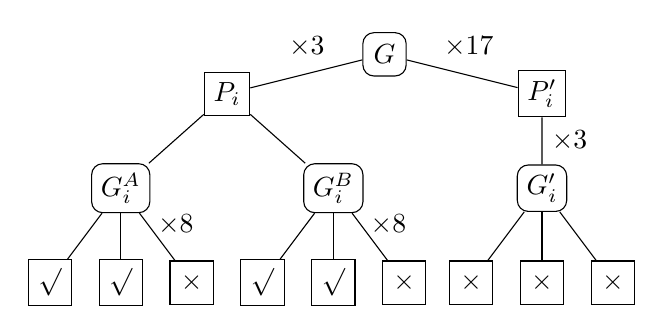
\begin{tikzpicture}[level distance=1.2cm]

\tikzstyle{planbox}=[draw,minimum height=0.55cm,minimum width=0.55cm]
\tikzstyle{goalbox}=[draw,rounded corners,minimum height=0.55cm,minimum width=0.55cm]

\tikzstyle{level 1}=[sibling distance=4cm,level distance=0.5cm] 
\tikzstyle{level 2}=[sibling distance=2.7cm,level distance=1.2cm]
\tikzstyle{level 3}=[sibling distance=.9cm]
\tikzstyle{level 4}=[sibling distance=1cm]

\node[goalbox] (T) {$G$}
   child[solid] {node[planbox] (1) {$P_i$}
      	child {node[goalbox] (11) {$G_i^A$}
			child {node[planbox] {$\surd$}
			}
			child {node[planbox] {$\surd$}
			}
			child {node[planbox] {$\times$}
				edge from parent node[right,near start] {$\times 8$}
			}
	  	}
      	child {node[goalbox] (11) {$G_i^B$}
			child {node[planbox] {$\surd$}
			}
			child {node[planbox] {$\surd$}
			}
			child {node[planbox] {$\times$}
				edge from parent node[right,near start] {$\times 8$}
			}
	  	}
	edge from parent node[above left, near start] {$\times 3$}
   }
   child[solid] {node[planbox] (2) {$P_i'$}
      child {node[goalbox] (22) {$G_i'$} 
	child {node[planbox] {$\times$}}
	child {node[planbox] {$\times$}}
	child {node[planbox] {$\times$}}
	edge from parent node[right] {$\times 3$}
	}
   edge from parent node[above right,near start] {$\times 17$}};

% \draw (T) -- (1) node (aux1) [coordinate,midway]{};
% \draw (T) -- (2) node (aux2) [coordinate,midway]{};
% \draw (aux1) .. controls +(0.3,-0.3) and +(-0.3,-0.3).. (aux2)
% 			node[midway,above] {OR};

% \draw (1) -- (11) node (aux21) [coordinate,midway]{};
% \draw (1) -- (12) node (aux23) [coordinate,midway]{};
% \draw (aux21) .. controls +(0.25,-0.25) and +(-0.25,-0.25).. (aux23)
% 			node[midway,above] {AND};

% \node[below left of=T,text width=2cm,xshift=-3cm] (label)
% 		{$P_i$: plan \\ $G_i$: goals \\ $SG_i$: sub-goals};
\end{tikzpicture}

\end{center}
\caption{Goal-plan tree hierarchical structure $\T_1$. To succeed, an agent is thus required to make three correct choices, including selecting $P$ at the top-level. The solutions to $2^3$ worlds are distributed evenly in the $3$ plans labelled $P_i$. \CL\ outperforms \BUL\ in this structure.}
\label{fig:T1}
\end{figure}


From our set of experiments, we have selected three hierarchical structures that
best illustrate the results that we have obtained, namely:
% %
\begin{description}
\item[(Tree $\T_1$; Figure~\ref{fig:T1})] For each world state, the
goal has a few plans that can succeed (plans $P_i$), but many other options of comparable
complexity that are bound to fail (plans $P_i'$). 
%%
Under this type of structure, an \CL-based agent will generally perform better 
than an agent using the learning \BUL\ approach.

\item[(Tree $\T_2$; Figure~\ref{fig:T2})] For each world state, the goal has
one plan that can succeed (plan $P$), and a few others that would fail.
However, the plan containing the solution is of substantially
higher-complexity\footnote{When we refer to plan complexity, we mean
the size of the expanded plan, as represented by the number of levels
of abstraction, and the numbers of goals at each level. The key issue
is number of abstraction levels. Abstract plans are not in themselves complex.}
%%
In this structure, a \BUL-based agent will outperform an \CL-based one.
% A structure in which \BUL\ is
% expected to have important advantages over \CL, since the latter may wrongly consider a
% top-level plan as a failing plan whereas there is a solution encoded
% under it. 

\item[(Tree $\T_3$; Figure~\ref{fig:T3})] This tree represents a ``balanced''
structure that ends up providing different advantages for both \BUL\ and \CL\ in
different parts of the tree.
\end{description}


% In summary, we found that whereas the agent performance under the \BUL\ and \CL\
% approaches is comparable on the first and third cases, the \BUL\ scheme provides
% substantial benefits in the second case. What is more important, if we consider
% agents that may choose not to consider a plan at all when its chances of success
% are believed very low, then the \CL\ approach collapses completely whereas the
% \BUL\ is robust enough to maintain performance.

% For lack of space, we shall only give the form of tree $\T_1$ and informally
% explain the characteristics of the other two.

Let us next discuss each of the plan-goal structures and how the performance of
\BUL-based and \CL-based agents compare.


Under a structure like $\T_1$, the agent basically has several options of
comparable complexity to resolve the top-level goal $G$ in a certain
world state. In $\T_1$ there are $20$ options.
However, most such options ($17$ in our example, plans $P_i'$)
inevitably lead to failure.  
% %
The benefit of using the \CL\ approach comes from the fact that the agent will
decrease the probability of selecting each of those $17$ failing plans as soon as
they fail for the first time. In contrast, \BUL\ requires multiple failed
experiences of each of those ``bad'' top-level options before decreasing their
probability of selection because each subgoal of each plan $P_i'$ must
be stable before that $P_i'$ is updated. 
%---to update the decision tree of each plan $P_i'$, \BUL\
%requires each of the three subgoals of that plan to be ``stable.''
% %%
The \CL\ agent did indeed perform better in our experiments, in that it
achieved better success rate earlier as shown in Figure~\ref{fig:T1_result}.
% %
The \CL\ approach reaches $50\%$ success after $1000$ iterations,
whereas it takes more than double that for \BUL\.
% %
Eventually, both approaches will yield optimal performance.\footnote{Optimal
performance amounts to a success rate of $81\%$, as the environment fails with
probability $.1$ for every (working) action and each successful execution
involves the performance of two actions (leaf plans consist of single actions).}


\begin{figure}[t]
\begin{center}
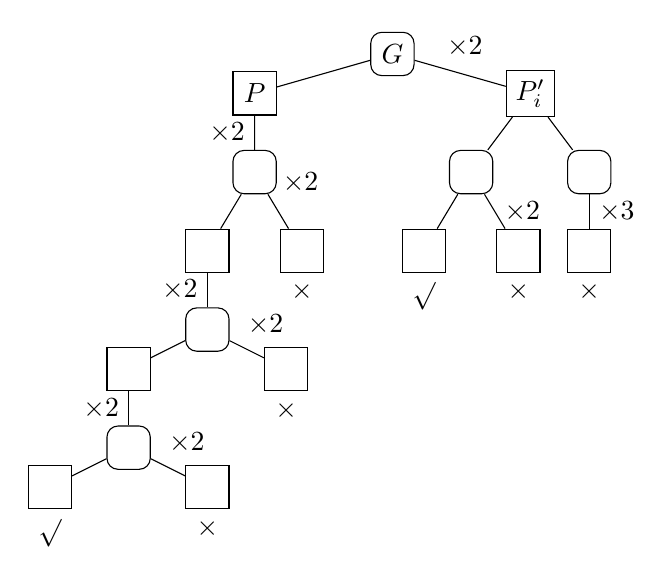
\begin{tikzpicture}[level distance=1.2cm]
\tikzstyle{txt}=[scale=.9]

\tikzstyle{succ}=[label=below:$\surd$]
\tikzstyle{fail}=[label=below:$\times$]


\tikzstyle{planbox}=[draw,minimum height=0.55cm,minimum width=0.55cm]
\tikzstyle{goalbox}=[draw,rounded corners,minimum height=0.55cm,minimum width=0.55cm]

\tikzstyle{level 1}=[sibling distance=3.5cm,level distance=0.5cm] 
\tikzstyle{level 2}=[sibling distance=1.5cm,level distance=1.0cm]
\tikzstyle{level 3}=[sibling distance=1.2cm,level distance=1.0cm]
\tikzstyle{level 4}=[sibling distance=1.2cm,level distance=1.0cm]
\tikzstyle{level 5}=[sibling distance=2.0cm,level distance=0.5cm]
\tikzstyle{level 6}=[sibling distance=1.2cm,level distance=1.0cm]
\tikzstyle{level 7}=[sibling distance=2.0cm,level distance=0.5cm]
\tikzstyle{level 8}=[sibling distance=1.2cm,level distance=1.0cm]

\node[goalbox] (T) {$G$}
   child[solid] {node[planbox] (1) {$P$}
      child {node[goalbox] (11) {\phantom{$G$}}
		child {node[planbox] {\phantom{$P$}}
			child {node[goalbox] {\phantom{$G$}}
				child {node[planbox] {\phantom{$P$}}
					child {node[goalbox] {\phantom{$G$}}
						child {node[planbox,succ] {\phantom{$P$}}}
						child {node[planbox,fail] {\phantom{$P$}}
							edge from parent node[above right,near start] {$\times 2$}
						}
						edge from parent node[left] {$\times 2$}
					}
				}
				child {node[planbox,fail] {$\phantom{P}$}
					edge from parent node[above right,near start] {$\times 2$}
				}
		               edge from parent node[left] {$\times 2$}
			}
		}
		child {node[planbox,fail] {\phantom{$P$}}
			edge from parent node[above right,near start] {$\times 2$}
		}
               edge from parent node[left] {$\times 2$}
	}
   }
   child[solid] {node[planbox] (2) {$P_i'$}
      	child {node[goalbox] (11) {\phantom{$G$}}
			child {node[planbox,succ] {$\phantom{P}$}}
			child {node[planbox,fail] {$\phantom{P}$} 
		               edge from parent node[right] {$\times 2$}
			}
	}
      	child {node[goalbox] {\phantom{$G$}}
			child {node[planbox,fail] {$\phantom{P}$} 
		               edge from parent node[right] {$\times 3$}
			}
	}
	edge from parent node[above right, near start] {$\times 2$}
};
\end{tikzpicture}



\end{center}
\caption{Goal-plan tree hierarchical structure $\T_2$. Successful execution requires numerous correct choices including $8$ correct action nodes. The solutions to $2^3$ worlds are in the plan labelled $P$. \BUL\ outperforms \CL\ in this structure.}
\label{fig:T2}
\end{figure}


\begin{figure*}[t]
\begin{center}
\subfigure[Structure $\T_1$]{\label{fig:T1_result}
%!TEX root = ../dsingh-aamas10-poster.tex
\begin{tikzpicture}[x= 0.008cm,y=9cm]
	\definecolor{darkblue}{rgb}{0.1,0.1,0.5}
	\definecolor{darkred}{rgb}{0.8,0.0,0.1}
    % Draw the axes and grid lines
    \draw[-] (0,0) -- (0,1) -- (2000,1) -- (2000,0) -- cycle; 
    \draw[-,thin, dotted, ystep=0.2, xstep=2000] (0,0) grid (2000,1);
    \foreach \x in {500, 1000, 1500}  \draw [-,xshift=0](\x,4pt) -- (\x,-1pt);
    \foreach \y in {0.0,0.2,0.4,0.6,0.8,1.0}  \draw [-,yshift=0](4pt,\y) -- (-1pt,\y);
    \foreach \x/\xtext in {500/500, 1000/1000, 1500/1500} \node at (\x,0) [below] {\xtext};
    \foreach \y/\ytext in {0.0,0.2,0.4,0.6,0.8,1.0}  \node at (0,\y) [left] {\ytext};
    \node at (0,1.15) {Success};
    \node at (1650,0.1) {Iterations};
    \draw[-,darkred] plot[mark=x,mark size=10,mark options={color=darkred}] 
			file {figs/data/test01v3gm.CP.tikzdata};
    \draw[-,darkblue] plot[mark=o,mark size=6,mark options={color=darkblue}] 
			file {figs/data/test01v3gm.SP.tikzdata};
    % Also draw the expected convergence: 0.9^4 actions=0.6561
    \draw[dashed,-,yshift=0](0,0.81) -- (2000,0.81);
	\node at (2300,0.5) {$\mathcal{T}1$};
\end{tikzpicture}

}
\qquad
\subfigure[Structure $\T_2$]{\label{fig:T2_result}
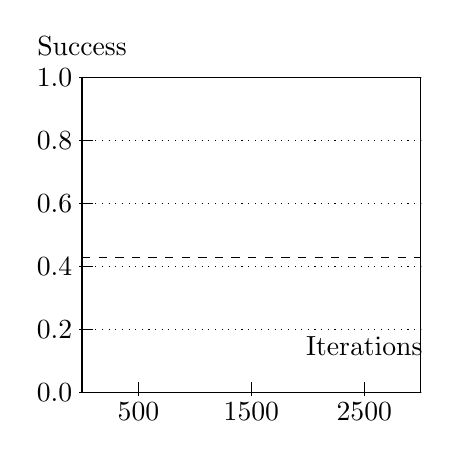
\begin{tikzpicture}[x=0.00143cm,y=4cm]
    % Draw the axes and grid lines
    \draw[-] (0,0) -- (0,1) -- (3000,1) -- (3000,0) -- cycle; 
    \draw[-,thin, dotted, ystep=0.2, xstep=3000] (0,0) grid (3000,1);
    \foreach \x in {500, 1500, 2500}  \draw [-,xshift=0](\x,4pt) -- (\x,-1pt);
    \foreach \y in {0.0,0.2,0.4,0.6,0.8,1.0}  \draw [-,yshift=0](4pt,\y) -- (-1pt,\y);
    \foreach \x/\xtext in {500/500, 1500/1500, 2500/2500} \node at (\x,0) [below] {$\xtext$};
    \foreach \y/\ytext in {0.0,0.2,0.4,0.6,0.8,1.0}  \node at (0,\y) [left] {$\ytext$};
    \node at (0,1.1) {Success};
    \node at (2500,0.15) {Iterations};
    \draw[-] plot[mark=triangle,gray,mark size=3,mark options={color=gray}] 
			file {data/test05v3gm.CP.tikzdata};
    \draw[-] plot[mark=o,gray,mark size=2,mark options={color=gray}] 
			file {data/test05v3gm.SP.tikzdata};
    % Also draw the expected convergence: 0.9^8 actions=0.43046
    \draw[dashed,-,yshift=0](0,0.43046) -- (3000,0.43046);

\end{tikzpicture}

}
\qquad
\subfigure[Structure $\T_3$]{\label{fig:T3_result}
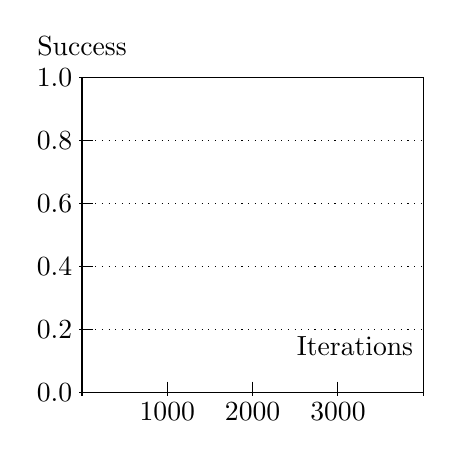
\begin{tikzpicture}[x=0.00108cm,y=4cm]
    % Draw the axes and grid lines
    \draw[-] (0,0) -- (0,1) -- (4000,1) -- (4000,0) -- cycle; 
    \draw[-,thin, dotted, ystep=0.2, xstep=4000] (0,0) grid (4000,1);
    \foreach \x in {0,1000,...,4000}  \draw [-,xshift=0](\x,4pt) -- (\x,-1pt);
    \foreach \y in {0.0,0.2,0.4,0.6,0.8,1.0}  \draw [-,yshift=0](4pt,\y) -- (-1pt,\y);
    \foreach \x/\xtext in {1000/1000, 2000/2000, 3000/3000} \node at (\x,0) [below] {$\xtext$};
    \foreach \y/\ytext in {0.0,0.2,0.4,0.6,0.8,1.0}  \node at (0,\y) [left] {$\ytext$};
    \node at (0,1.1) {Success};
    \node at (3200,0.15) {Iterations};
    \draw[-] plot[mark=triangle,gray,mark size=3,mark options={color=gray}] 
			file {data/testImpactvars.CP.tikzdata};
    \draw[-] plot[mark=o,gray,mark size=2,mark options={color=gray}] 
			file {data/testImpactvars.SP.tikzdata};

\end{tikzpicture}

}
\caption{Agent performance under \BUL\ (circles) and \CL\ (triangles) schemes.
Each point represents results from $5$ experiment runs using a moving average of $100$ samples.}
\end{center}
\end{figure*}


Let us now analyse the goal-plan tree $\T_2$ shown in Figure~\ref{fig:T2}.
% %
Under such a structure, all successful executions are encoded in a complex plan, in our
case plan $P$. Other options that the agent may have (e.g., plans $P_i'$) are of
less complexity, but do not lead to solutions for resolving the
goal.\footnote{This is an extreme case for illustrative purposes. Of
course the simpler plans $P_i'$ would, in a real program, lead to a
solution in some world states or it would not make sense to include
them. The same effect would however arise if most world states had
solutions only in a complex plan branch.}
% %
Because the plan containing the solution, namely $P$, is fairly
complex, there are many ways the agent may fail when exploring the
decomposition of $P$. The agent needs to make several correct choices to
obtain a successful execution.
% %
Although we expected \BUL\ to yield better agent performance than \CL, the
difference was enormous in our experiments. Figure \ref{fig:T2_result} shows that
while the \BUL\ approach achieves optimal performance, which amounts to slightly
over $40\%$ rate of success, in around $300$ iterations, the \CL\ scheme,
requires close to $2500$ execution experiences. The reason is clear: since there
are more chances to fail plan $P$ initially, \CL\ marks this plan as ``bad,''
compared with the non-working plans $P_i'$. On the other hand, \BUL\ would not
jump to the conclusion that $P$ is a ``bad'' plan even when failing it, since it
is aware that decisions made below $P$ were not sufficiently informed. Consequently,
plan $P$ will continue to be explored with \emph{equal} likelihood to plans
$P_i'$.
% %
This structure shows exactly the problem discussed in the previous
section, namely, the drawbacks of assuming a plan is a bad option just because it
happened to fail, without consideration of the confidence in the choices
made below the plan in question.


Finally, consider the hierarchical structure $\T_3$ depicted in Figure
\ref{fig:T3}.
% %
In this case, the top-level goal $G$ has four relevant plans, which are all
``complex,'' that is, they all have several levels and multiple goals and plans.
However, given a world state, only one particular path in this hierarchy will
lead to a successful execution (of course, for different states, different
top-level plans may apply). Among other things, this means that at the top-level
the agent needs to select the right plan given the current world state. All 
other plans are bound to eventually fail.
% %
We argue that this is a common feature found in many BDI agent applications, in
that even though the agent has been programmed with several strategies for
resolving a goal, each one is crafted to cover uniquely a particular subset of
states. In other words, these are systems with low \emph{know-how} overlap.
% %
With respect to the two learning approaches we are considering, structure $\T_3$
provides advantages for both of them, in different parts of the tree. The \CL\
scheme is expected to learn faster the inadequacy of the non-working top-level
programs, whereas the \BUL\ would better explore, and find a solution, within the
working top-level plan. This balance was corroborated in our experiments, in
which both type of agents experienced comparable performance; see Figure
\ref{fig:T3_result}.




\subsection{Plan Applicability and Optimality}

So far, we have assumed that the agent, considers all relevant plans
for a goal as also \emph{applicable}, even though some may have a very
low chance of success.
% %
This implies that, in contrast with standard BDI systems, our extended
learning BDI framework will \emph{always} select a plan among the relevant
options.
% %
Because executing a plan is often not cost-free in real systems, it is likely
that an adequate plan selection mechanism would in fact \emph{not} execute plans
with too low a probability of success. This, in turn, implies that the system
may, at some point, decide to fail a goal without even trying it, if it
considers that the high likelihood of failure does not justify the
cost of attempting any of the relevant plans.
%cost of failing at that point is preferable to expected
%benefits of executing some available plan.
%%
This is exactly what standard BDI systems do. When no applicable plan
is found for a certain event goal, that event goal is failed right away.


To understand the impact of applicability in our BDI learning framework, we
modified the probabilistic plan selection so that the agent does not consider
plans whose chances of success are deemed below a threshold; in our case we set
this threshold to $0.2$.
% %
For simplicity, we  removed the non-determinism in the model of the
environment so that actions either fail or succeed in each world state.

%The difference between \CL-based and \BUL-based agents performance when run with
%an applicability threshold could be striking
% %
Using the structure $\T_3$ we found that whereas the \BUL\ scheme maintains its
performance (and in fact may slightly improve due to truly failing leaf plans
being ruled out earlier), the \CL\ approach may not able to learn at all and
could end up eventually failing the top-level goal \emph{always}. This is
reported in Figure \ref{fig:T3_result} (dotted lines).

The explanation for this undesirable behavior under \CL\ is as follows.
% %
Initially, the agent tries all top-level plans for the top-level goal, including
the ones containing potential successful executions. Because of their complexity,
the chance of finding a successful execution immediately is very low, and most
executions fail initially. With each failure, \CL\ decreases the feasibility of
all plans tried, including the top-level one.  After several failures, all plans
for the top-level goal eventually go below the applicability threshold of the
system (including the ``good'' plans). When that happens, the system has no more
applicable plans for the goal and will therefore fail it always.
% %
This behavior does not arise in the original system, because even if all plans
perform very poorly, the agent would always pick one anyway, the successful path
would be eventually be found, and the context decision trees of the plans
associated with such a path would then start ``recovering.''


The reason why \BUL\ exhibits more robust behaviour here is that false negative
execution runs (i.e., failing executions of a plan that do encode a successful
execution) will \emph{not} be recorded.
% %
The \BUL\ approach relies on a \emph{confidence} test---stability---that checks
whether we are sufficiently well informed to trust that the current failure is
indicative of future attempts.
% %
In the next section, we explore an alternative approach to confidence 
that takes account of how sure we are of the decision tree when we use
it, rather than attempting, via stability, to ensure that we only
record results that we are confident in.
%that can be combined with \CL\ (or \BUL) and is able to overcome the
%weaknesses shown here.
